% Example LaTeX commands to generate a NorthStar justification ps/pdf file
\documentclass[a4paper, 11pt]{article}
\usepackage{graphics,graphicx}
\oddsidemargin=-0.54cm
\evensidemargin=-0.54cm
\topmargin=-1.2cm
\textwidth=17cm
\textheight=25cm
\pagestyle{empty}
\begin{document}

%%Lensing%%
\begin{figure}[tbh]
\centering
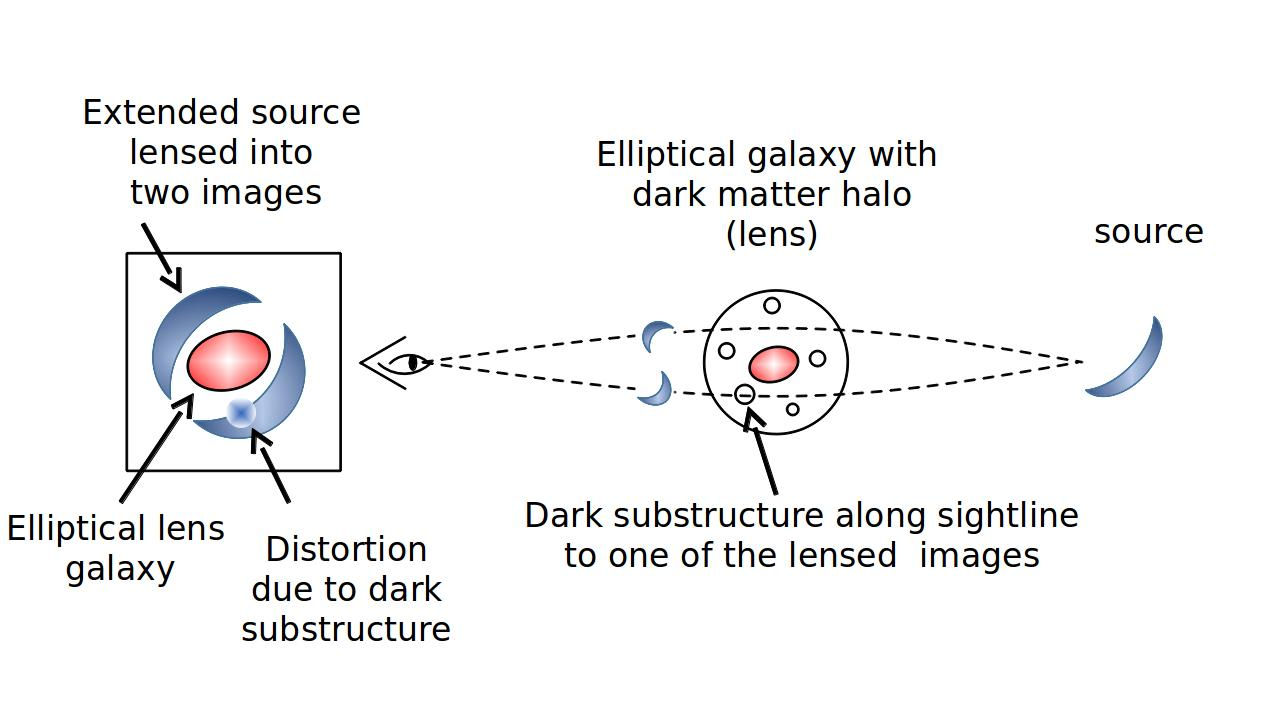
\includegraphics[scale=0.3]{Figure_lensing.jpg}
\caption{Schematic illustration of gravitational millilensing as a probe of dark halo substructure. A foreground galaxy with a dark matter halo produces two macroimages of a background light source. A subhalo (or other substructure) located in the dark halo intercepts the path of one of these macroimages and produces a small-scale distortion (millilensing) in its surface brightness distribution. Whereas morphological anomalies intrinsic to the source should be mimicked in both macroimages, millilensing will affect each macroimage differently, and typically turn up just in one image.}
\end{figure}

%%Spectrum%%
%\begin{figure}[b]
%\centering
%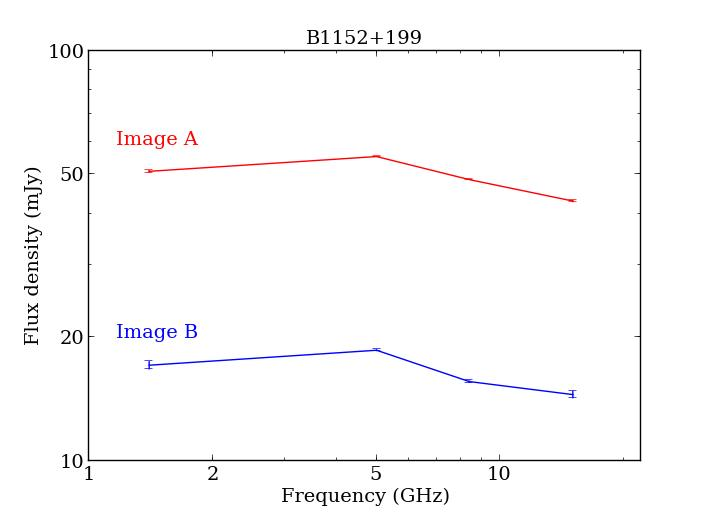
\includegraphics[scale=0.4]{Figure_spectrum.jpg}
%\caption{Schematic illustration of gravitational millilensing as a probe of dark halo substructure. A foreground galaxy with a dark matter halo produces two macroimages of a background light source. A subhalo (or other substructure) located in the dark halo intercepts the path of one of these }
%\end{figure}


%%EVN 2002%%
\begin{figure}[tbh]
\centering
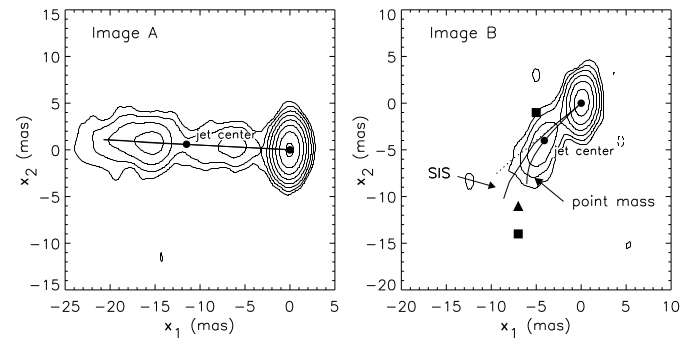
\includegraphics[scale=0.75]{Figure_2002.jpg}
\caption{The VLBA 5-GHz maps (Rusin et al. 2002; beam $3.6 \times 1.9$ mas$^2$) of the two macroimages of B1152+199, overlaid with lens models from Metcalf (2002). The slight curvature of the jet in the right panel (image B) is attributed to millilensing by a substructure located close to this macroimage. In the absence of such substructure, the jet in the right macroimage would follow the path given by the dotted, straight line (a poor fit to the data). The two curved paths are produced when different forms of substructures are introduced. The lowermost curve is given by a point-mass substructure (IMBH) of mass $\sim 10^5$–-$10^7 M_\odot$ located at the position of the triangle. The intermediate curve is reproduced by two SIS substructures (squares) with poorly constrained masses. Metcalf (2002) emphasizes that while the jet bending indicates some form of millilensing, the substructure solution (in terms of substructure position and mass) to these data is by no means unique.}
\end{figure}

%%EVN 2012%%
\begin{figure}[tbh]
\centering
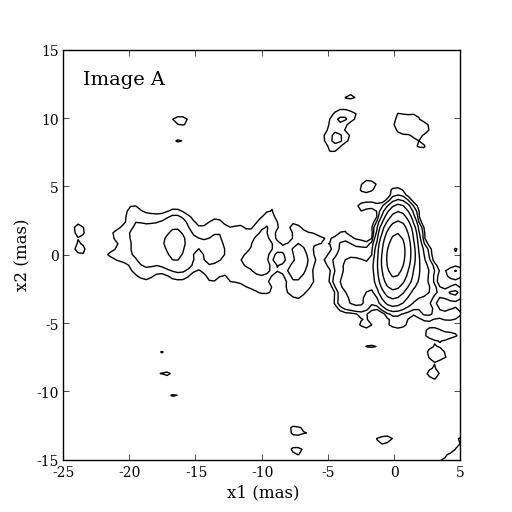
\includegraphics[scale=0.5]{Figure_2012A.jpg}
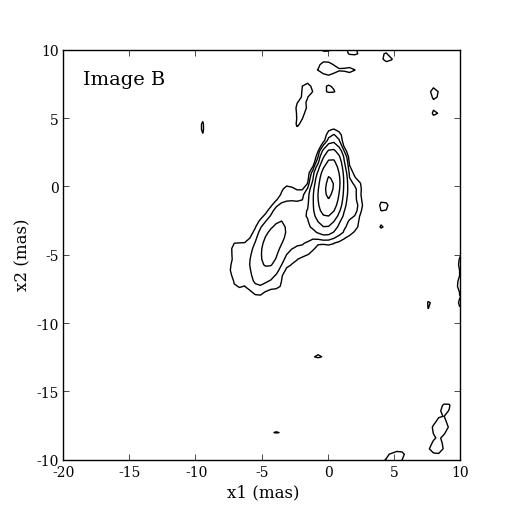
\includegraphics[scale=0.5]{Figure_2012B.jpg}
\caption{The archival EVN 5-GHz maps (beam $3.8 \times 1.4$ mas$^2$) of the two macroimages of B1152+199. Contour levels are the same as in figure 2; the lowest contour is 3 times the map rms noise in figure 2 ($75 \mu$ Jy beam$^{-1}$) and each contour level increases by a factor of 2. The slight curvature of the jet in the right panel (image B) seems to be unchanged over 10 years. This, in addition to the much shorter ($\approx 40$--$70$ days) gravitational time delay of the system, suggests that the curvature cannot be due to jet precession.}
\end{figure}
\end{document}
